
\index{Optics|textbf}

This section describes advanced neutron optical
components such as supermirrors and guides.
A description of the reflectivity of a supermirror is found
in section~\ref{s:mirror}.

\section{Mirror: The single mirror}
\label{s:mirror}
\index{Optics!Mirror plane}
\component{Mirror}{System}{$l$, $h$, $m$}{$R_0, Q_c, W, \alpha$}{validated, no gravitation support}

The component {\bf Mirror}
models a single rectangular neutron mirror plate. It can be used
as a sample component or to \textit{e.g.}~assemble a complete neutron guide by putting multiple
mirror components at appropriate locations and orientations in the
instrument definition, much like a real guide is build from individual
mirrors.

In the local coordinate system, the mirror lies in the first quadrant of the
$x$-$y$ plane, with one corner at $(0,0,0)$.

The input parameters of this component are
the rectangular mirror dimensions $(l, h)$
and the values of $R_0, m, Q_c, W$, and $\alpha$ for the mirror reflectivity.
As a special case, if $m=0$ then the reflectivity is zero for all $Q$,
\textit{i.e.}\ the surface is completely absorbing.

This component may produce wrong results with gravitation.

\subsection{Mirror reflectivity}
\label{ss:mirrorreflect}
To compute the reflectivity of the supermirrors, we use an empirical
formula derived from experimental data \cite{pb_241_50},
see Fig.~\ref{f:reflectivity}. The reflectivity is given by
\begin{equation} \label{e:Rmirror}
  R = \left\{
    \begin{array}{ll}
      R_0 & \textrm{if $Q \leq Q_{\rm c}$} \\
      \frac{1}{2}R_0(1 - \tanh[(Q - m Q_{\rm c})/W])(1-\alpha(Q-Q_{\rm c}))
         & \textrm{if $Q > Q_{\rm c}$}
    \end{array}
  \right.
\end{equation}

Here $Q$ is the length of the scattering vector (in \AA$^{-1}$)
defined by
\begin{equation} \label{e:reflectivity}
Q = |{\bf k}_{\bf i} - {\bf k}_{\bf f}|
  = \frac{m_{\rm n}}{\hbar} |{\bf v}_{\bf i} - {\bf v}_{\bf f}|,
\end{equation}
$m_{\rm n}$ being the neutron mass.
The number $m$ in (\ref{e:Rmirror}) is a parameter determined by
the mirror materials,
the bilayer sequence, and the number of bilayers.
As can be seen, $R=R_0$ for $Q < Q_{\rm c}$, where $Q_{\rm c}$ is the
critical scattering wave vector for a single layer of the mirror
material. At higher values of $Q$, the reflectivity starts falling
linearly with a slope $\alpha$ until a "soft cut-off" at $Q = m Q_{\rm c}$.
The width of this cut-off is denoted $W$. See the example reflection curve in
figure~\ref{f:reflectivity}.

It is {\bf important} to notice that when $m < 1$, the reflectivity remains constant at $R=R_0$ up to $q=Qc$, and \emph{not} $m.Q_c$. This means that $m < 1$ parameters behave like $m=1$ materials.

\subsection{Algorithm}
The function of the component can be described as
\begin{enumerate}
\item Propagate the neutron ray to the plane of the mirror.
\item If the neutron trajectory intersects the mirror plate, it is
reflected, otherwise it is left untouched.
\item Reflection of the incident velocity
${\bf v}_{\rm i} = (v_x,v_y,v_z)$
gives the final velocity ${\bf v}_{\rm f} = (v_x,v_y,-v_z)$.
\item Calculate $Q=2 m_{\rm n} v_z / \hbar$.
\item The neutron weight is adjusted with the amount $\pi_i = R(Q)$.
\item  To avoid spending large amounts of computation time on very low-weight
neutrons, neutrons for which the reflectivity is lower than about
$10^{-10}$ are ABSORB'ed.
\end{enumerate}

\begin{figure}
  \begin{center}
    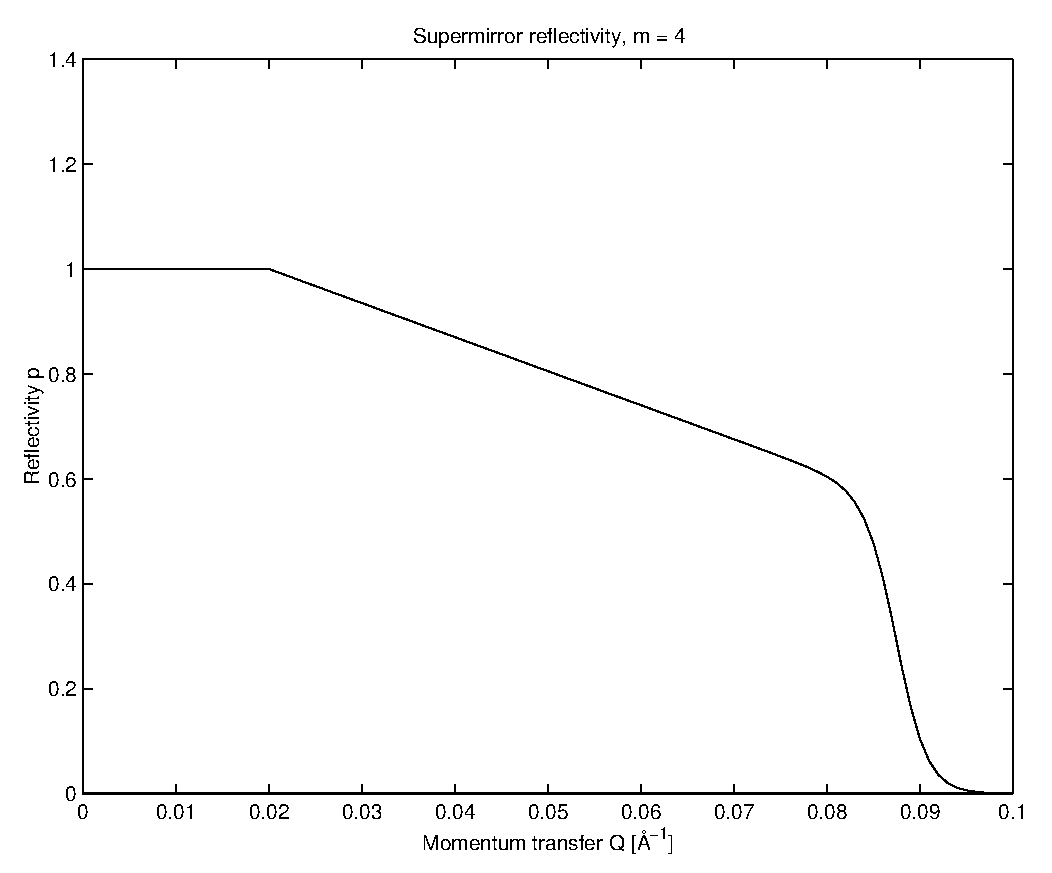
\includegraphics[width=0.6\textwidth]{figures/supermirror.eps}
  \end{center}
\caption{A typical reflectivity curve for a supermirror,
Eq.~(\protect\ref{e:reflectivity}). The used values are
$ m=4$, $R_0=1$, $Q_{\rm c} = 0.02$~\AA$^{-1}$, $\alpha = 6.49$~\AA,
$ W=1/300$~\AA$^{-1}$.
}
\label{f:reflectivity}
\end{figure}

\newpage

\section{Guide: The guide section}
\index{Optics!Straight guide}

\component{Guide}{System}{$w_1, h_1$, $w_2, h_2$, $l$, $m$}{$R_0, Q_c, W, \alpha$}{validated, no gravitation support}

The component {\bf Guide}
models a guide tube consisting of four flat mirrors. The
guide is centered on the $z$ axis with rectangular entrance and exit
openings parallel to the $x$-$y$ plane. The entrance has the dimensions
$(w_1,h_1)$ and placed at $z=0$. The exit is of dimensions $(w_2,h_2)$
and is placed at $z=l$ where $l$ is the guide length. See
figure~\ref{f:guide}.
The reflecting properties are given by the values of
$R_0, m, Q_c, W$, and $\alpha$, as for {\bf Mirror}.

{\bf Guide} may produce wrong results with gravitation support.
Use {\bf Guide\_gravity} (section \ref{s:guide_gravity}) in this case.
For a more general guide simulation, see {\bf Guide\_channeled}
in section~\ref{s:channeled_guide}.

\begin{figure}
  \begin{center}
    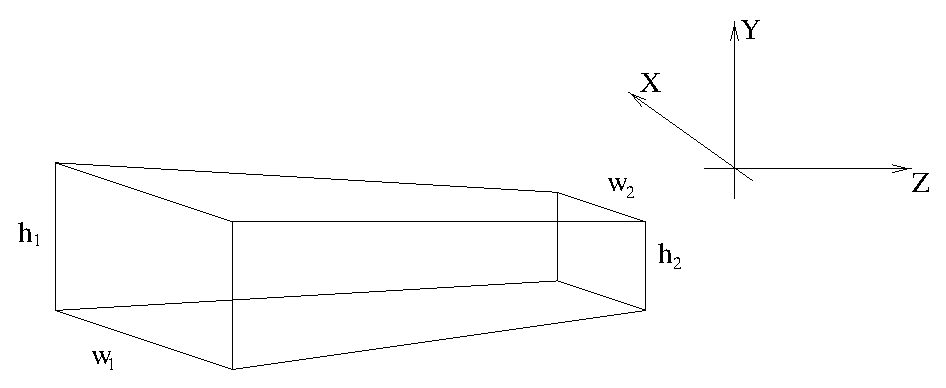
\includegraphics[width=0.7\textwidth]{figures/guide1.eps}
  \end{center}
\caption{The geometry used for the guide component.}
\label{f:guide}
\end{figure}

\subsection{Guide geometry and reflection}
For computations on the guide geometry, we define the planes of the four
guide sides by giving their normal vectors (pointing into the guide)
and a point lying in the plane:
$$
\begin{array}{rclcrcl}
{\bf n}^v_1 &=& (l, 0, {(w_2 - w_1) / 2})
     & & {\bf O}^v_1 &=& (- w_1 / 2, 0, 0) \\
{\bf n}^v_2 &=& (-l, 0, {(w_2 - w_1) / 2})
     & & {\bf O}^v_2 &=& (w_1 / 2, 0, 0) \\
{\bf n}^h_1 &=& (0, l, {(h_2 - h_1) / 2})
     & & {\bf O}^h_1 &=& (0, - h_1 / 2, 0) \\
{\bf n}^h_2 &=& (0, -l, {(h_2 - h_1) / 2})
     & & {\bf O}^h_2 &=& (0, h_1 / 2, 0) \\
\end{array}
$$
In the following, we refer to an arbitrary guide side by its origin
{\bf O} and normal {\bf n}.

With these definitions, the time of intersection of the neutron with a
guide side can be computed by considering the projection onto the
normal:
\begin{equation}
t^\alpha_\beta = \frac{({\bf O}^\alpha_\beta - {\bf r}_0) \cdot {\bf n}^\alpha_\beta}
  {{\bf v} \cdot {\bf n}^\alpha_\beta}  ,
\end{equation}
where $\alpha$ and $\beta$ are indices for the different guide walls,
assuming the values (h,v) and (1,2), respectively.
For a neutron that leaves the guide directly through the guide exit we have
\begin{equation}
t_{\rm exit} = \frac{l - z_0}{v_z}
\end{equation}

The reflected velocity ${\bf v}_{\rm f}$ of the neutron with incoming velocity
${\bf v}_{\rm i}$ is computed by the formula
\begin{equation}
 {\bf v}_{\rm f} =
  {\bf v}_{\rm i}
   - 2{{\bf n} \cdot {\bf v}_{\rm i} \over {|{\bf n}|^2}} {\bf n}
\end{equation}
This expression is arrived at by again considering the projection onto
the mirror normal (see figure~\ref{f:guidereflect}). The reflectivity of the
mirror is taken into account as explained in section~\ref{s:mirror}.

\begin{figure}
  \begin{center}
    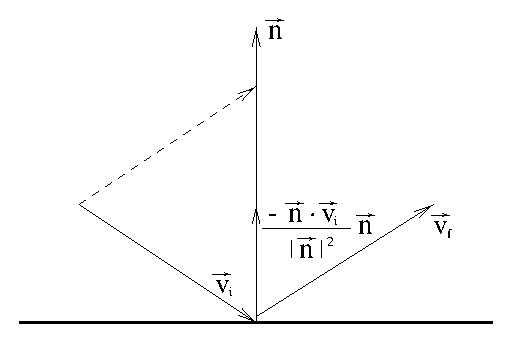
\includegraphics[width=0.5\textwidth]{figures/guide2.eps}
  \end{center}
\caption{Neutron reflecting from mirror. ${\bf v}_{\rm i}$ and
${\bf v}_{\rm f}$ are the initial and final velocities, respectively,
and {\bf n} is a vector normal to the mirror surface.}
\label{f:guidereflect}
\end{figure}

\subsection{Algorithm}
\begin{enumerate}
\item The neutron is initially propagated to the $z = 0$ plane of the
guide entrance.
\item If it misses the entrance, it is ABSORB'ed.
\item Otherwise, repeatedly compute the time of intersection with the
four mirror sides and the guide exit.
\item The smallest positive $t$ thus
found gives the time of the next intersection with the guide (or in the
case of the guide exit, the time when the neutron leaves the guide).
\item Propagated the neutron ray to this point.
\item Compute the reflection from the side.
\item Update the neutron weight factor by the amount $\pi_i = R(Q)$.
\item Repeat this process until the neutron leaves the guide.
\end{enumerate}

There are a few optimizations possible here to avoid redundant
computations. Since the neutron is always inside the guide during the
computations, we always have
$({\bf O} - {\bf r}_0) \cdot {\bf n} \leq 0$.
Thus $t \leq 0$ if ${\bf v} \cdot {\bf n} \geq 0$, so in this case
there is no need to actually compute $t$. Some redundant computations
are also avoided by utilizing symmetry and the fact that many
components of {\bf n} and {\bf O} are zero.

\newpage

\section{Guide\_channeled: A guide section component with multiple channels}
\label{s:channeled_guide}
\index{Optics!Guide with channels (straight, non focusing)}

\component{Guide\_channeled}{System}{$w_1, h_1$, $w_2, h_2$, $l$, $k$, $m_x, m_y$}{$d, R_0, Q_{cx}, Q_{cy}, W, \alpha_x, \alpha_y$}{validated, no gravitation support}

The component {\bf Guide\_channeled} is a more complex variation of {\bf Guide}
described in the previous section. It allows the specification
of different supermirror parameters for the horizontal and vertical
mirrors, and also implements guides with multiple channels as used in
neutron bender devices. By setting the $m$ value of the supermirror
coatings to zero, nonreflecting walls are simulated;
this may be used for a very detailed simulation of a Soller collimator,
see section~\ref{collimator-linear}.

The input parameters are $w_1$, $h_1$, $w_2$, $h_2$, and $l$
to set the guide dimensions as for {\bf Guide}
(entry window, exit window, and length);
$k$ to set the number of channels; $d$ to set the thickness of the
channel walls; and $R_0$, $W$, $Q_{cx}$, $Q_{cy}$, $\alpha_x$, $\alpha_y$,
$m_x$, and $m_y$ to set the supermirror parameters as described under {\bf Guide}
(the names with \textit{x} denote the vertical mirrors,
and those with \textit{y} denote the horizontal ones).

\subsection{Algorithm}
The implementation is based on that of {\bf Guide}.
\begin{enumerate}
\item Calculate the channel which the neutron will enter.
\item Shift the $x$ coordinate so that the channel can be simulated
as a single instance of the {\bf Guide} component.
\item (do the same as in {\bf Guide}.)
\item Restore the coordinates when the
neutron exits the guide or is absorbed.
\end{enumerate}

\subsection{Known problems}\index{Bugs}
\begin{itemize}
\item This component may produce wrong results with gravitation support.
Use Guide\_gravity (section \ref{s:guide_gravity}) in this case.
\item The focusing channeled geometry (for $k > 1$ and different
values of $w_1$ and $w_2$) is buggy
(wall slopes are not computed correctly, and the component 'leaks' neutrons).
\end{itemize}
\newpage

\section{Guide\_gravity: A guide with multiple channels and gravitation handling}
\label{s:guide_gravity}
\index{Optics!Guide with channels and gravitation handling (straight)}

\component{Guide\_gravity}{System}{$w_1, h_1$, $w_2, h_2$, $l$, $k$, $m$}{$d, R_0, Q_c, W, \alpha$, wavy, chamfers, $k_h$, $n$, $G$}{validated, {\bf with} gravitation support}

This component is a variation of {\bf Guide\_channeled}
(section \ref{s:channeled_guide}) with the ability to handle
gravitation effects and functional channeled focusing geometry.
Channels can be specified in two dimensions,
producing a 2D array ($k, k_h$) on smaller guide channels.

Waviness effects, supposed to be randomly distributed
(\emph{i.e.} non-periodic waviness)
can be specified globally, or for each part of the guide section.
Additionally, chamfers
may be defined the same way.
Chamfers originate from the substrate manufacturing, so that operators do not harm themselves with cutting edges. Usual dimensions are about tens of millimeters. They are treated as absorbing edges around guide plates, both on the input and output surfaces, but also aside each mirror.

The straight section of length $l$ may be divided into $n$ bits of same length
within which chamfers are taken into account.

To activate gravitation support, either select the \MCS\ gravitation support,
or set the gravitation field strength $G$ (e.g. -9.81 on Earth).

\section{Bender: a bender model (non polarizing)}
\index{Optics!Bender (non polarizing)}

\component{Bender}{Philipp Bernhardt}{$r, W_{in},l,w,h $}{$k,d,R_{0[a,i,s]},\alpha_{[a,i,s]},m_{[a,i,s]},Q_{c[a,i,s]},W_{[a,i,s]}$}{partly validated, no gravitation support}

The Bender component is simulating an ideal curved neutron guide (bender). It is bent to the negative X-axis and behaves like a parallel guide in the Y axis. Opposite curvature may be achieved by a $(0,0,180)$ rotation (along Z-axis).

Bender radius $r$, entrance width $w$ and height $h$ are required parameters. To define the length, you may either enter the deviation angle $W_{in}$ or the length $l$. Three different reflectivity profiles $R_0,Q_c,W,m,\alpha$ can be given (see section~\ref{s:mirror}): for outer
walls (index $a$), for inner walls (index $i$) and for the top and bottom walls (index $s$).

To get a better transmission coefficient, it is possible to split the bender into $k$ channels which are separated by partitions with the thickness of $d$. The partitioning walls have the same coating as the exterior walls.

Because the angle of reflection doesn't change, the routine
calculates the reflection coefficent for the concave and, if necessary, for the convex wall only onces, together with the number of reflections.
Nevertheless the exact position, the time, and the divergence is calculated at the end of the bender, so there aren't any approximations.

The component is shown \emph{straight} on geometrical views (mcdisplay/Trace), and the next component may be placed directly at distance $r.W_{in} = l$ \emph{without} rotation.

Results have been compared succesfully with analytical formula in the case of an ideal reflection and cross-checked with the program \verb+haupt+.

An other implementation of the Bender is available as the contributed component Guide\_curved.

\section{Curved guides}
\index{Optics!Curved guides (polygonal model)}

Real curved guides are usually made of many straight elements (about 1 m long) separated with small gaps (e.g. 1 mm). Sections of about 10 m long are separated with bigger gaps for accessibility and pumping purposes.

We give here an example description of such a section. Let us have a curved guide of total length $L$, made of $n$ elements with a curvature radius $R$. Gaps of size $d$ separate elements from each other. The rotation angle of individual straight guide elements is $\alpha_z = (L+d)/R*180/\pi$ in degrees.

In order to build an independent curved guide section, we define \verb+Arm+ components at the begining and end of it.
\begin{verbatim}
COMPONENT CG_In = Arm() AT (...)

COMPONENT CG_1  = Guide_gravity(l=L/n, ...)
AT (0,0,0) RELATIVE PREVIOUS

COMPONENT CG_2  = Guide_gravity(l=L/n, ...)
AT (0,0,L/n+d) RELATIVE PREVIOUS
ROTATED (0, (L/n+d)/R*180/PI, 0) RELATIVE PREVIOUS
...
COMPONENT CG_Out = Arm() AT (0,0,L/n) RELATIVE PREVIOUS
\end{verbatim}
The \verb+Guide+ component should be duplicated $n$ times by copy-paste, but changing the instance name, e.g. CG\_1, CG\_2, ..., CG\_n.

An implementation of a continuous curved guide has been contributed as component Guide\_curved.

